\chapter{Experimental Results}

\section{The Data}

\noindent The aim of this thesis is to implement, and then fine-tune, a CNN to classify voxels of chest computerised tomography (CT) scan as being either in the part of the heart called the atrium or outside of it. The atrium is the two entry point of the blood into the heart. It is composed of two chambers: a right one which recovers blood returning to the heart to complete the cardiovascular cycle through the body, and a left one receiving blood coming back from the lungs after being oxygenated and purified of toxins.\\

\noindent The data from which the training and testing datasets are generated comprise 27 CT scans. CT scans are 3 dimensional grey scale images, generally of size 480*480*50, generated via computers combining many X-ray images taken from different angles to produce cross-sectional images of specific body parts. They are stored as DICOM files, DICOM standing for Digital Imaging and Communications in Medicine which is a standard for handling, storing, printing, and transmitting information in medical imaging. Each has been segmented by trained radiologists at St Thomas's hospital, the results of which are stored in Nearly Raw Raster Data (NRRD) files, a standard format for storing raster data. These are 3D arrays of the same dimension as their corresponding CT scan with each entry being either a 1 or 0 indicating whether its corresponding voxel belongs in the atrium or not. 

\section{Generating the datasets: The Tri-Planar Method}

\begin{figure}
\centering
\label{tri-planar}
\begin{minipage}{0.45\textwidth}
\centering
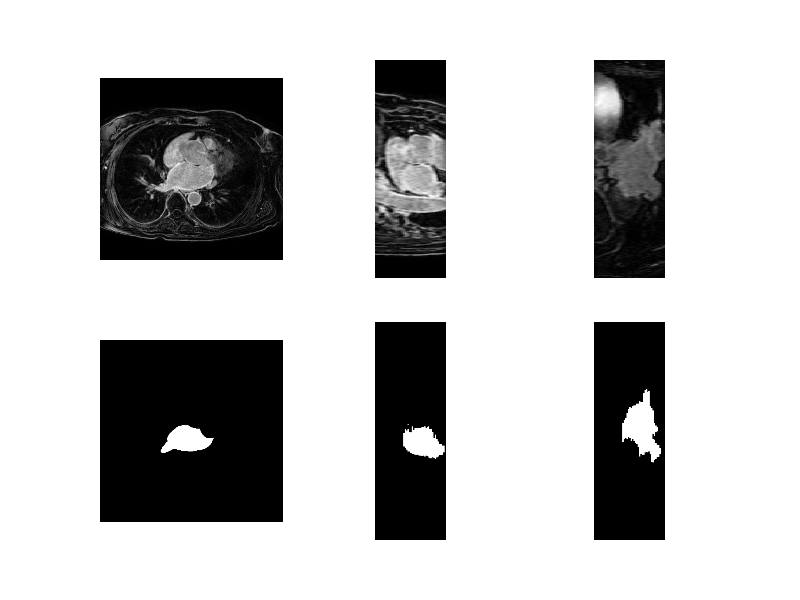
\includegraphics[trim=3cm 1.5cm 3cm 1.5cm, clip=true, height=60mm]{Chapter3/example_slice.png}
\end{minipage}\hfill
\begin{minipage}{0.45\textwidth}
\centering
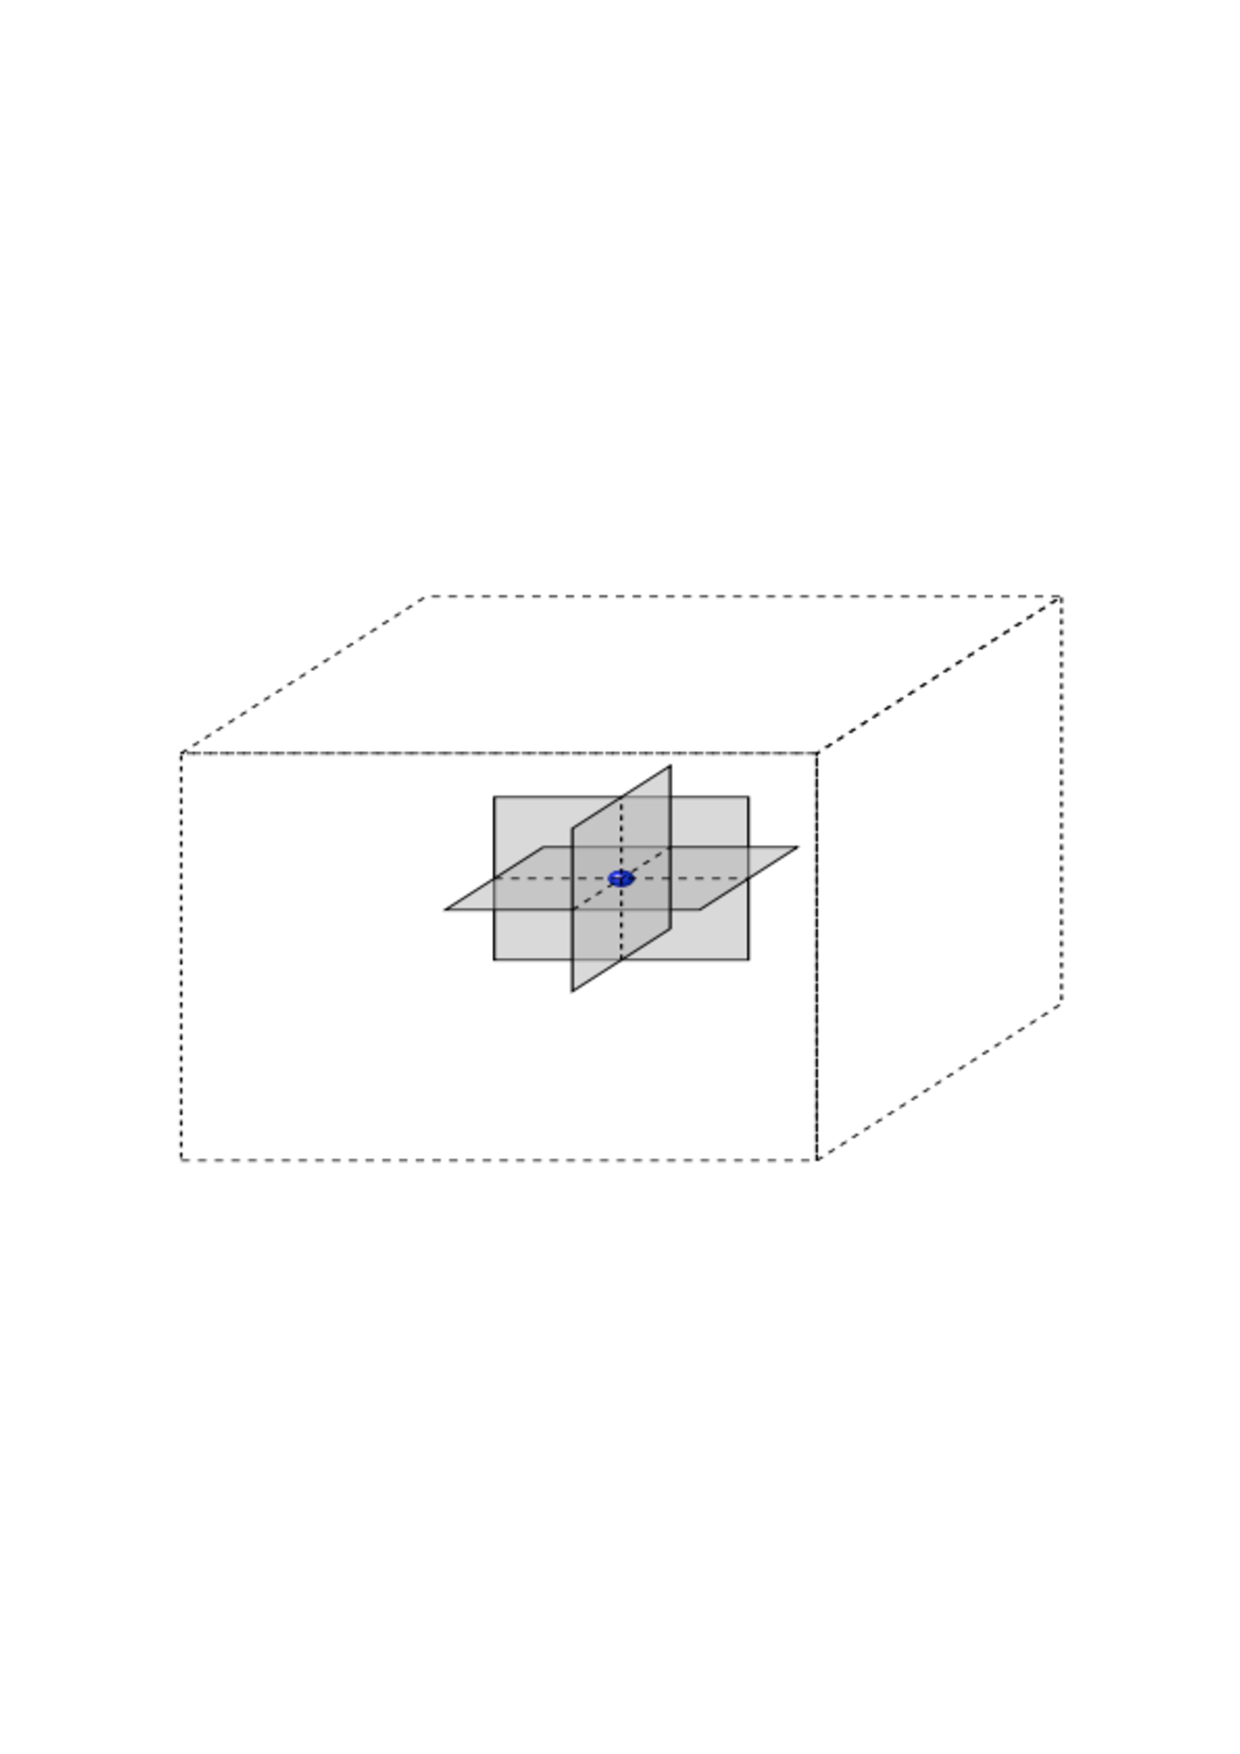
\includegraphics[trim=2cm 8cm 2cm 8cm, clip=true, height=60mm]{Chapter3/triplanar.pdf}
\end{minipage}
\caption{Left: grey scale slices from a CT scan taken in the transversal, saggital and coronal planes. Right: illustration of the triplanar}
\end{figure}

\noindent Classifying the voxels requires building a set of input vectors each containing enough local and global information to allow the neural network to learn effectively. One way of providing 3 dimensional information is to use the tri-planar method. This consists in generating 3 perpendicular square patches of a given dimension in the transversal, saggital and coronal planes centred at the voxel of interest as shown in Figure \ref{tri-planar}. This technique has been found to give competitive results compared to using 3D patches while being much more computationally and memory efficient \citep{knee_cartilage}. In addition, we use a multi-scale approach as in \citep{DBLP:journals/corr/BrebissonM15}, where we add 3 more input channels composed of compressed patches that are originally 5 times larger than the above set of patches, but resized to be of the same size as the first 3 input patches to provide global information about the surroundings of the concerned voxel.\\

\noindent Each patch is fed into a different input channel of the CNN to a total of 6 channels. The outputs of those channels are then feed as inputs to a set of connected layers itself connected to a classifying layer.

\section{Implementation Details}

\subsection{Libraries}

\noindent Our CNNs were implemented using Torch, an open-source library aiming to provide a Matlab-like environment for scientific computing in Lua, along with a number of dependent libraries (nn, cunn, cudnn, fbcunn) which facilitate the training of neural networks on single and multiple GPUs. In addition, we use Python and a number of its libraries to handle all the logistics ranging from generating the datasets to producing plots of segmentation results.

\subsection{Computer facilities}

\noindent The training of the CNNs were conducted alternatively on one of 2 multi-GPU clusters, named montana-nvidia and montana-k80, kindly provided by Prof. Montana. montana-nvidia consists of 24 cores with 129 Gb of memory connected to two NVIDIA Tesla K40m and two Tesla K20Xm while montana-k80 on the other hand has 56 cores with 258 Gb of memory supported by 8 of NVIDIA's Testla K80. 

\section{Model Selection}

\subsection{General approach for model selection}

\noindent The purpose of this section is to find a good set of hyper-parameters fro our CNN. To that end, we allocate 20 of the 27 CT scans for generating the training set and the remaining 7 for generating the validation set. The training set is composed of 400000 training examples equally divided among the training CT scans, half being in the atrium and the other half outside it. The validation set is composed of 200000 examples equally divided among the testing CT scans. Furthermore at the end of training, each model fully segments a test CT scan from the testing set to provide performance statistics. In particular, from this segmentation image, we evaluate the model's sensitivity (the percentage of correctly classified atrium voxels), specificity (the percentage of correctly classified non-atrium voxels), and overall classification rate also known as the Dice coefficient, calculated by evaluating the proportion of correctly classified voxels in the segmented image. As 98\% of the CT scan is composed of non-atrium voxels, the Dice coefficient is overwhelmingly influenced by the specificity. We will conduct our model selection by selectively choosing hyper-parameters that optimise the Dice coefficient while having a reasonable sensitivity in the regions of 80 to 90\%.\\

Additionally, mask images are generated from 3 transversal slices in the segmented CT. The masks are formed by overlaying the grey scale CT scan image with colours representing the error status of the classification of a given voxel. They provide a visual representation of the performance of the models. The colour codes are:

\begin{itemize}
	\item Green: correctly classified atrium voxel.
	\item Blue: correctly classified non-atrium voxel.
	\item Red: incorrectly classified atrium voxel.
	\item Pink: incorrectly classified non-atrium voxel.
\end{itemize}

\noindent We start off our model selection with a CNN comprised of an input layer with 6 channels of patches of size 32*32, 2 convolutional layers with 32 and 64 feature maps respectively and a max pooling filter of size $2 \times 2$, 2 fully connected layers with 1000 and 500 hidden units each respectively, and a logsoftmax output layer giving the log probabilities of the voxel belonging to either classes. The training parameters are composed of a learning rate of 0.01, a momentum rate set to 0, and a mini-batch size set to 6000 examples. In addition, the negative log likelihood criterion provides the error measure during training. We will be varying in turn the following hyper-parameters while at each stage keeping the others constant.\\

\begin{itemize}
	\item the number of convolutional layers.
	\item the number of connected layers.
	\item the number of feature maps in the chosen number of convolutional layers.
	\item the number of hidden units in the chosen number of connected layers.
	\item the learning rate.
	\item the momentum.
	\item the type of activation function (ReLU, Tanh or Sigmoid).
\end{itemize}

\subsection{Varying the Number of Convolutional Layers}

\noindent To select the number of convolutional layers, we train 4 CNNs with architectures starting with the following convolutional layers:

\begin{itemize}
	\item Input (6*32*32) => Conv layer (32*28*28) => 2*2 MaxPooling filter (32*14*14) 
	\item Input (6*32*32) => Conv layer (32*28*28) => 2*2 MaxPooling filter (32*14*14) => Conv layer (64*10*10) => 2*2 MaxPooling filter (64*5*5)
	\item Input (6*32*32) => Conv layer (32*28*28) => Conv layer (32*24*24) => 2*2 MaxPooling filter (32*12*12) => Conv layer (64*8*8) => 2*2 MaxPooling filter (64*4*4)
	\item Input (6*32*32) => Conv layer (32*28*28) => Conv layer (32*24*24) => 2*2 MaxPooling filter (32*12*12) => Conv layer (64*8*8) => Conv layer (64*4*4) => 2*2 MaxPooling filter (64*2*2)
\end{itemize}

\noindent The values in parentheses indicate the number and dimensions of the feature maps at each layer. The following table gives the results for each of these architectures trained over 100 epochs.\\

\begin{tabular}{cccccc}
\rowcolor[HTML]{C0C0C0} 
        \# Conv Layers & \begin{tabular}[c]{@{}c@{}}Dice \\ training set\end{tabular} & \begin{tabular}[c]{@{}c@{}}Dice \\ testing set\end{tabular} & Sensitivity & Specificity & \begin{tabular}[c]{@{}c@{}}Dice \\ test CT scan\end{tabular} \\ \hline
1  & 0.959                                                        & 0.956                                                       & 0.913       & 0.970       & 0.969                                                        \\ 
2  & 0.958                                                        & 0.961                                                       & 0.734       & 0.989       & 0.984                                                        \\ 
3  & 0.956                                                        & 0.960                                                       & 0.762       & 0.987       & 0.983                                                        \\ 
4  & 0.959                                                        & 0.956                                                       & 0.881       & 0.973       & 0.972                                                       
\end{tabular}\\

\noindent The table above presents the key test statistics across the 4 architectures considered. The architecture with the best test Dice coefficient is the one with 2 convolutional layer, closely followed by the one with 3 convolutional layers, with dice coefficients of 0.984 and 0.983 respectively. These two architectures give low sensitivities of 0.734 and 0.762 respectively. However the architectures with 1 and 4 convolutional layers yield significantly lower Dice coefficients of 0.969 and 0.972 respectively, despite a much greater sensitivity of 0.913 and 0.881. \\

\begin{figure}
\centering
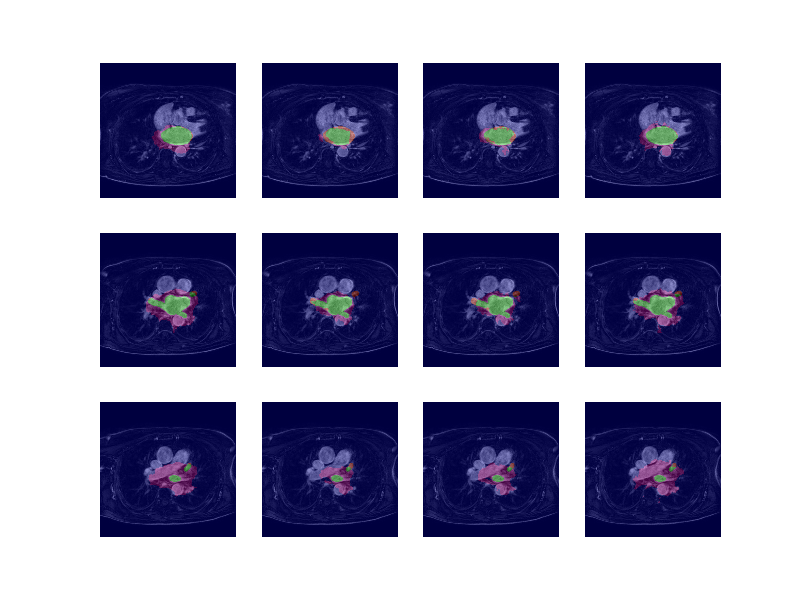
\includegraphics[trim=2.5cm 1.5cm 2cm 1.5cm, clip=true, height=80mm, width=150mm]{Chapter3/mask_results_varying_number_of_convolutional_layers.png}
\caption{Masks for varying number of convolutional layers}
\end{figure}

\noindent Figure whatever brings a visual element to this comparison. The first and fourth columns correspond to segmentations by the architectures with 1 and 4 convolutional layers respectively. These show much larger pink patches, corresponding to higher rates of false positives than the other two columns but with smaller red regions corresponding to lower rates of false negatives, corroborating the story told by the sensitivity and specificity in the table above. There is not much difference between the masks of the second and third layers.\\

\noindent We choose to go with the architecture with the highest Dice coefficient at this stage and thus select an architecture with 2 convolutional layers. 

\subsection{varying number of connected layers}

\noindent Having settled on an architecture with 2 convolutional layers, we now train 3 CNNs with 1, 2, and 3 fully connected layers each starting with 1000 hidden units and halving the number of hidden units for each additional layer. Hence the CNN with 3 fully connected layers has 1000, 500, and 250 hidden units in each layer respectively. The results are shown in the following table.\\

\begin{tabular}{cccccc}
\rowcolor[HTML]{C0C0C0} 
             \begin{tabular}[c]{@{}c@{}}\# Connected \\ Layers \end{tabular} & \begin{tabular}[c]{@{}c@{}}Dice \\ training set\end{tabular} & \begin{tabular}[c]{@{}c@{}}Dice \\ testing set\end{tabular} & Sensitivity & Specificity & \begin{tabular}[c]{@{}c@{}}Dice \\ test CT scan\end{tabular} \\ \hline
1  & 0.957                                                        & 0.959                                                       & 0.887       & 0.972       & 0.971                                                        \\ 
2  & 0.958                                                        & 0.961                                                       & 0.856       & 0.974       & 0.972                                                        \\ 
3  & 0.953                                                        & 0.951                                                       & 0.915       & 0.967       & 0.966                                                       
\end{tabular}\\

\begin{figure}
\centering
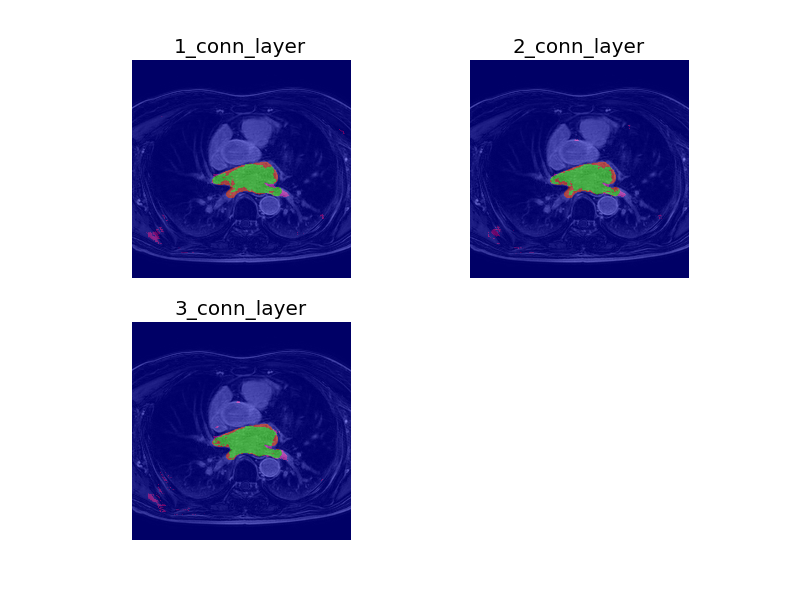
\includegraphics[trim=2.5cm 1.5cm 2cm 1.5cm, clip=true, height=80mm, width=150mm]{Chapter3/mask_results_varying_number_of_connected_layers.png}
\caption{Masks for varying number of connected layers}
\end{figure}

\noindent All three architectures have similar performances on the test CT scan. The architectures with 1 and 2 connected layers in particular that have the highest Dice coefficients of the three have marginally different specificities of 0.972 and 0.974 respectively. The discrepancies between their sensitivities are somewhat more pronounced at 0.887 and 0.856 respectively. Figure whatever similarly shows very little differences in the colour profile of the masks for all three architectures. Thus it seems that adding extra connected layers doesn't make much difference to the performance of the classifier and hence we opt for having 1 fully connected layer in our final architecture.

\subsection{varying number of feature maps}

\noindent We now focus on finding the right number of feature maps for the convolutional layers. In order to keep the computation comparable between the 2 layers, we set the number of feature maps in the second layer to be twice that of the first layer. We tried configurations with the first layer having 16, 32, and 64 feature maps. The summary of the results are shown below.\\

\begin{tabular}{cccccc}
\rowcolor[HTML]{C0C0C0} 
          \begin{tabular}[c]{@{}c@{}}\# Feature \\ Maps \end{tabular}  & \begin{tabular}[c]{@{}c@{}}Dice \\ training set\end{tabular} & \begin{tabular}[c]{@{}c@{}}Dice \\ testing set\end{tabular} & Sensitivity & Specificity & \begin{tabular}[c]{@{}c@{}}Dice \\ test CT scan\end{tabular} \\ \hline
 16  & 0.956                                                        & 0.953                                                       & 0.919       & 0.967       & 0.966                                                        \\ 
 32  & 0.957                                                        & 0.958                                                       & 0.894       & 0.972       & 0.970                                                        \\ 
 64  & 0.959                                                        & 0.958                                                       & 0.904       & 0.971       & 0.970                                                        
\end{tabular}\\

\noindent Yet again there is not much difference between the performance of all three architectures. The two with the highest test Dice coefficients are the ones with the first layer having 32 and 64 feature maps both at 0.970 and very similar sensitivities around 0.9. The one with 16 feature maps yields a slightly lower specificity of 0.967 but a higher sensitivity of 0.919 with an overall lower Dice coefficient of 0.966. The masks show slight differences in the first row of images, with a larger pink region for the 16 feature map architecture. These statistics don't justify having twice as many feature maps, we opt for having 32 feature maps i the first layer of the architecture.

\begin{figure}
\centering
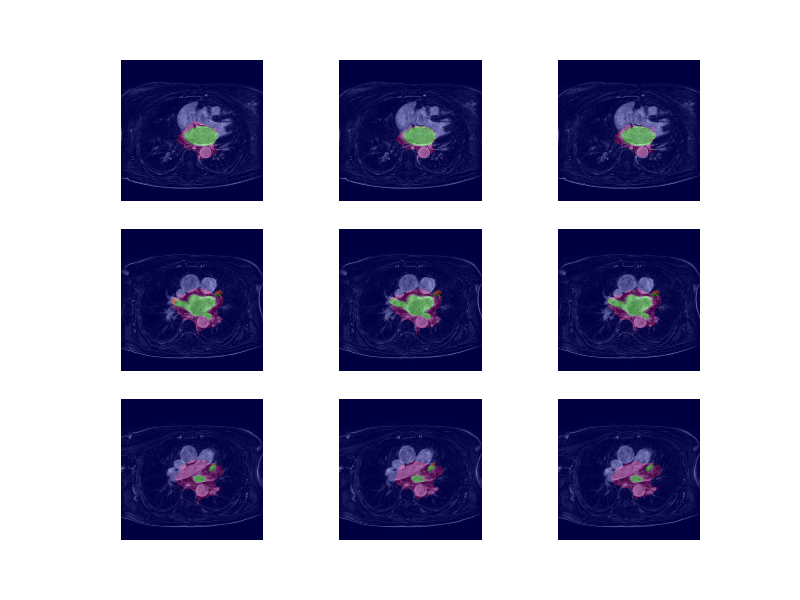
\includegraphics[trim=2.5cm 1.5cm 2cm 1.5cm, clip=true, height=80mm, width=150mm]{Chapter3/mask_results_varying_number_of_feature_maps.png}
\caption{Masks for varying number of feature maps}
\end{figure}

\subsection{varying the number of hidden units}

\noindent We now vary the number of hidden units in the connected layer, trying 100, 200, 500, 1000 hidden units. \\

\begin{tabular}{cccccc}
\rowcolor[HTML]{C0C0C0} 
                 \begin{tabular}[c]{@{}c@{}}\# Hidden \\ Units \end{tabular} & \begin{tabular}[c]{@{}c@{}}Dice \\ training set\end{tabular} & \begin{tabular}[c]{@{}c@{}}Dice \\ testing set\end{tabular} & Sensitivity & Specificity & \begin{tabular}[c]{@{}c@{}}Dice \\ test CT scan\end{tabular} \\ \hline
100   & 0.956                                                        & 0.958                                                       & 0.879       & 0.972       & 0.97                                                         \\ 
200   & 0.958                                                        & 0.957                                                       & 0.878       & 0.971       & 0.97                                                         \\ 
500   & 0.957                                                        & 0.955                                                       & 0.894       & 0.97        & 0.968                                                        \\ 
1000  & 0.957                                                        & 0.958                                                       & 0.892       & 0.972       & 0.97                                                        
\end{tabular}\\

\noindent Here the test statistics across all 4 architectures are very similar with a specificity around 0.97 and a sensitivity around 0.89. Given the tie, we select the simpler model with 100 hidden units.

\begin{figure}
\centering
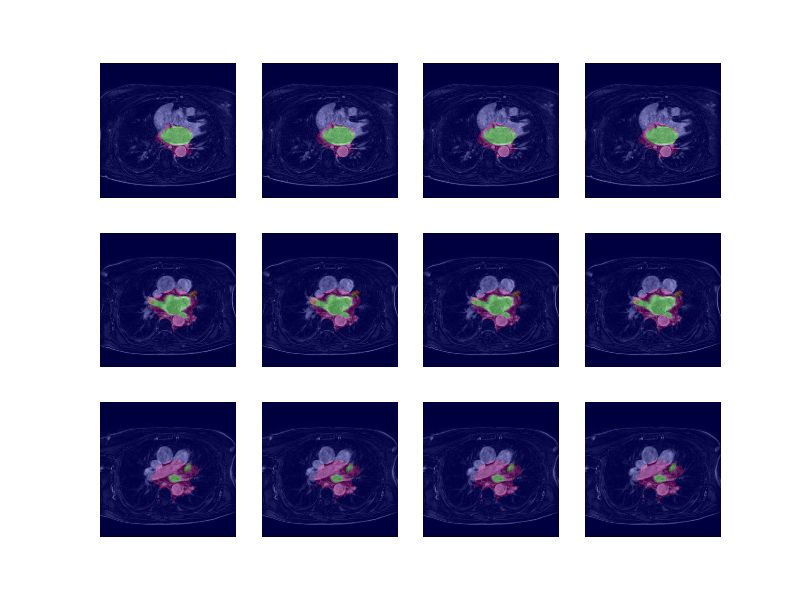
\includegraphics[trim=2.5cm 1.5cm 2cm 1.5cm, clip=true, height=80mm, width=150mm]{Chapter3/mask_results_varying_number_of_hidden_units.png}
\caption{Masks for varying number of hidden units}
\end{figure}

\subsection{varying the learning rate}

\noindent Tried different learning rates: 0.01, 0.05, 0.1, 0.5. Huge improvement as we increase the learning rate. A learning rate of 1 doesn't converge. We take LR = 0.5.

\begin{tabular}{cccccc}
\rowcolor[HTML]{C0C0C0} 
\begin{tabular}[c]{@{}c@{}}Learning\\ Rate\end{tabular} & \begin{tabular}[c]{@{}c@{}}Dice \\ training set\end{tabular} & \begin{tabular}[c]{@{}c@{}}Dice \\ testing set\end{tabular} & Sensitivity & Specificity & \begin{tabular}[c]{@{}c@{}}Dice \\ test CT scan\end{tabular} \\ \hline
\rowcolor[HTML]{FFFFFF} 
LR 0.01                                                 & 0.956                                                        & 0.957                                                       & 0.885       & 0.971       & 0.97                                                         \\
\rowcolor[HTML]{FFFFFF} 
LR 0.05                                                 & 0.97                                                         & 0.97                                                        & 0.915       & 0.977       & 0.976                                                        \\ 
\rowcolor[HTML]{FFFFFF} 
LR 0.1                                                  & 0.973                                                        & 0.973                                                       & 0.916       & 0.98        & 0.978                                                        \\
\rowcolor[HTML]{FFFFFF} 
LR 0.5                                                  & 0.982                                                        & 0.973                                                       & 0.932       & 0.982       & 0.981                                                       
\end{tabular}

\begin{figure}
\centering
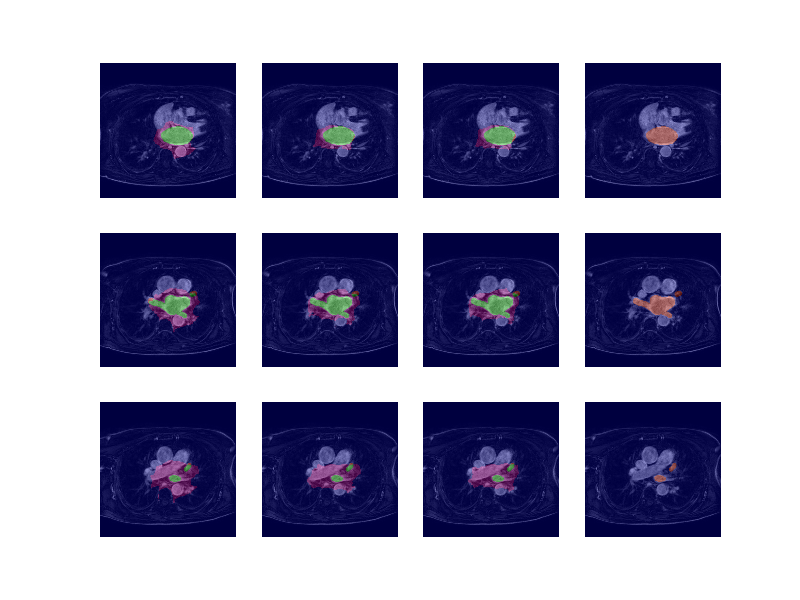
\includegraphics[trim=2.5cm 1.5cm 2cm 1.5cm, clip=true, height=80mm, width=150mm]{Chapter3/mask_results_varying_learning_rate.png}
\caption{Mask for varying learning rate.}
\end{figure}

\subsection{varying the momentum}

\noindent Tried different momentums: 0, 0.01, 0.05, 0.1, 0.5, 1.

\begin{tabular}{cccccc}
\rowcolor[HTML]{C0C0C0} 
Momentum & \begin{tabular}[c]{@{}c@{}}Dice \\ training set\end{tabular} & \begin{tabular}[c]{@{}c@{}}Dice \\ testing set\end{tabular} & Sensitivity & Specificity & \begin{tabular}[c]{@{}c@{}}Dice \\ test CT scan\end{tabular} \\ \hline
\rowcolor[HTML]{FFFFFF} 
0        & 0.982                                                        & 0.973                                                       & 0.906       & 0.982       & 0.981                                                        \\ 
\rowcolor[HTML]{FFFFFF} 
0.05     & 0.979                                                        & 0.973                                                       & 0.916       & 0.98       & 0.979                                                        \\ 
\rowcolor[HTML]{FFFFFF} 
0.1      & 0.983                                                        & 0.976                                                       & 0.9         & 0.984         & 0.982                                                        \\
\rowcolor[HTML]{FFFFFF} 
0.5      & 0.985                                                        & 0.981                                                       & 0.83        & 0.988        & 0.985                                                       
\end{tabular}

\begin{figure}
\centering
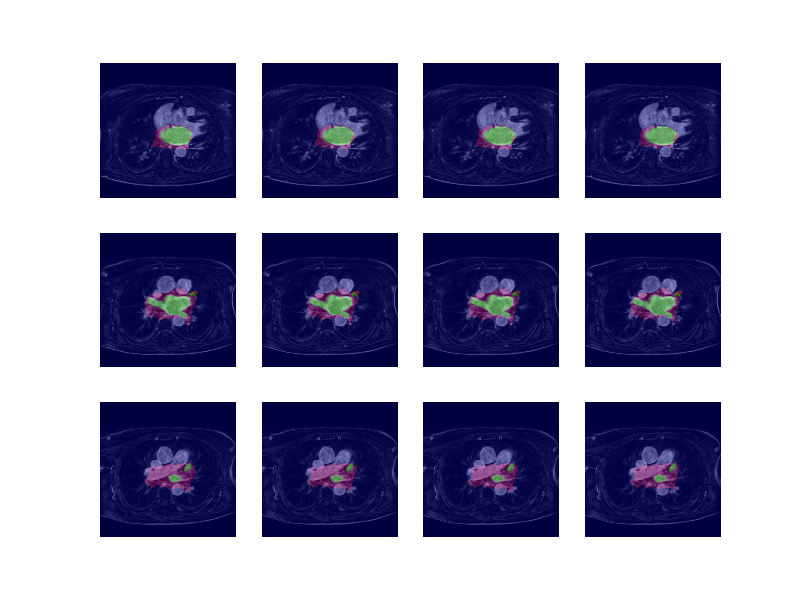
\includegraphics[trim=2.5cm 1.5cm 2cm 1.5cm, clip=true, height=80mm, width=150mm]{Chapter3/mask_results_varying_momentum.png}
\caption{Masks for varying momentum}
\end{figure}

\subsection{varying the activation function}

\noindent We experimented with different types of activation function: ReLU, Tanh, Sigmoid. Doing it with ReLU is better...\\

\begin{tabular}{cccccc}
\rowcolor[HTML]{C0C0C0} 
\begin{tabular}[c]{@{}c@{}}Activation\\ Function\end{tabular} & \begin{tabular}[c]{@{}c@{}}Dice \\ training set\end{tabular} & \begin{tabular}[c]{@{}c@{}}Dice \\ testing set\end{tabular} & Sensitivity & Specificity & \begin{tabular}[c]{@{}c@{}}Dice \\ test CT scan\end{tabular} \\ \hline
\rowcolor[HTML]{FFFFFF} 
ReLU                                                          & 0.984                                                        & 0.978                                                       & 0.87        & 0.986       & 0.984                                                        \\
\rowcolor[HTML]{FFFFFF} 
Tanh                                                          & 0.973                                                        & 0.972                                                       & 0.934       & 0.98        & 0.979                                                        \\
\rowcolor[HTML]{FFFFFF} 
Sigmoid                                                       & 0.958                                                        & 0.958                                                       & 0.941       & 0.968       & 0.967                                                       
\end{tabular}

\begin{figure}
\centering
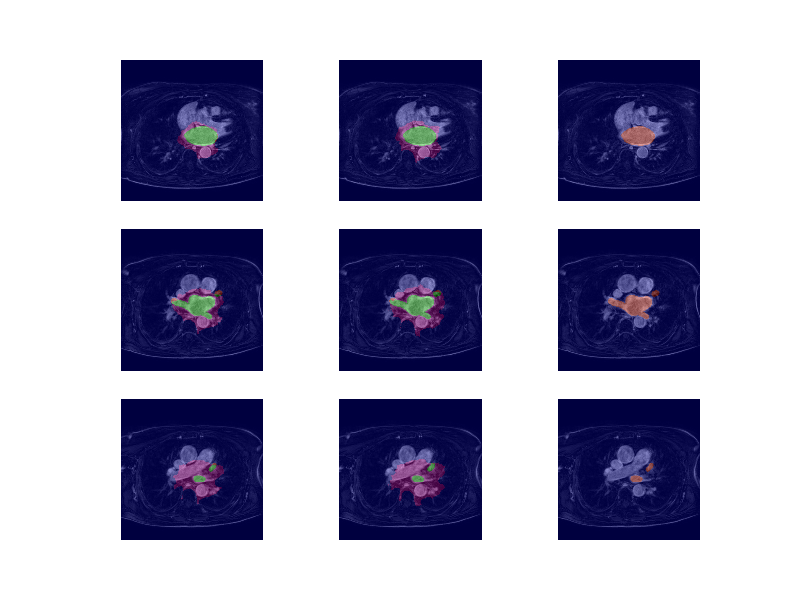
\includegraphics[trim=2.5cm 1.5cm 2cm 1.5cm, clip=true, height=80mm, width=150mm]{Chapter3/mask_results_varying_activation_function.png}
\caption{Masks for varying activation function}
\end{figure}

\subsection{varying datasets type}

\noindent The first thing we investigate is the sampling method for obtaining the training set. In order to increase the number of non-atrium training examples lying near the boundaries where we expect most of the classification errors to lie, we construct a rectangular area which contains the atrium. The atrium box is constructed by going through all the coordinates of the voxels labeled as being in the atrium, picking the minimum and maximum values in each of the coordinate planes, and possibly adding some padding, this procedure gives us a box containing the atrium. \\

\noindent We train our base CNN on 3 sampling procedures with no atrium box, i.e. all the non-atrium training examples are sampled randomly uniformly, a small atrium box constructed by the procedure above with a padding of 5 pixels in the x and y coordinate directions and of 1 pixel in the z coordinate direction, and finally a large atrium box with a padding of 30 pixels in the x and y coordinates and of 5 pixels in the z coordinate.\\

\noindent The results of the three training runs are shown in Figure whatever. From the testing dice coefficient plot, we get a better classification rate with sampling using an atrium box than no atrium box and particularly with the smaller atrium box. In the segmentation mask, sampling with no atrium box clearly yields more errors in the proximity of the atrium but none away from it whereas there are some errors far away from the atrium from the models trained with the atrium box sampling procedure. This is a consequence of the sampling procedures in both cases. Sampling with an atrium box would naturally yield better segmentation results near the atrium as the proportion of training examples is much higher in those regions than without an atrium box around it.\\

\begin{tabular}{cccccc}
\rowcolor[HTML]{C0C0C0} 
\begin{tabular}[c]{@{}c@{}}Training\\ Dataset\end{tabular} & \begin{tabular}[c]{@{}c@{}}Dice \\ training set\end{tabular} & \begin{tabular}[c]{@{}c@{}}Dice \\ testing set\end{tabular} & Sensitivity & Specificity & \begin{tabular}[c]{@{}c@{}}Dice \\ test CT scan\end{tabular} \\ \hline
\rowcolor[HTML]{FFFFFF} 
No Atrium Box                                              & 0.982                                                        & 0.978                                                       & 0.881       & 0.986       & 0.984                                                        \\
\rowcolor[HTML]{FFFFFF} 
Small Atrium Box                                           & 0.96                                                         & 0.987                                                       & 0.838       & 0.994       & 0.991                                                        \\
\rowcolor[HTML]{FFFFFF} 
Large Atrium Box                                           & 0.963                                                        & 0.983                                                       & 0.871       & 0.989       & 0.987                                                       
\end{tabular}

\subsection{varying the data size}

\begin{figure}
\centering
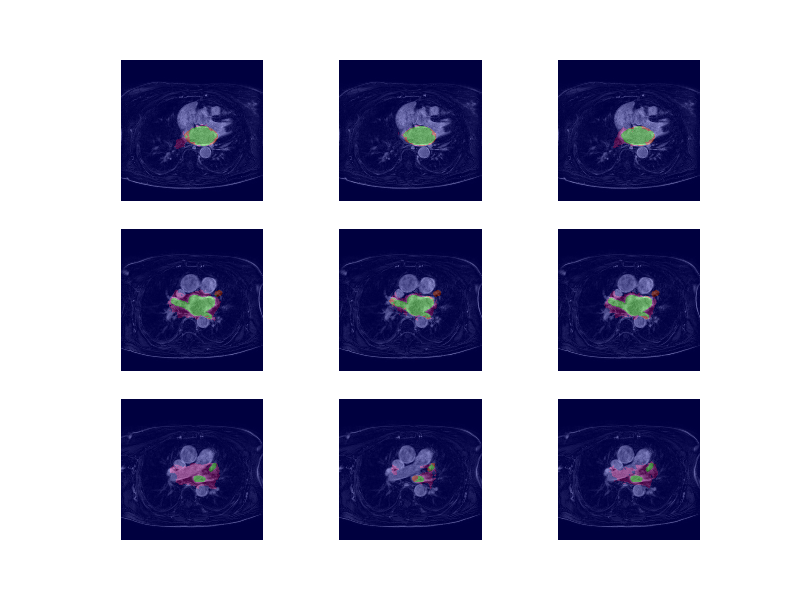
\includegraphics[trim=2.5cm 1.5cm 2cm 1.5cm, clip=true, height=80mm, width=150mm]{Chapter3/mask_results_varying_training_dataset.png}
\caption{Masks for varying training dataset}
\end{figure}

\noindent Tried a number of dataset sizes: 400000, 1000000, 3000000






